%\documentclass[paper,twocolomn]{geophysics}
\documentclass[manuscript]{geophysics}
%\documentclass[manuscript,endfloat]{geophysics}
\usepackage{amsmath,amssymb,amsfonts,graphicx,subfigure,bm,yfonts,hyperref,cleveref,xcolor}
\usepackage{rotating}
%\usepackage[outdir=./]{epstopdf}

\usepackage{multirow}


%%%%%%%%%                              DEFINITIONS START

\def\cpar{$C_{ij},\rho$ parameterization~}
\def\hpar{h-parameterization~}

\newcommand{\todo}[1]{{\textbf {\color{red} #1}}}
\newcommand{\done}[1]{{\bf {\color{green} #1}}}
\newcommand{\connect}{{\textbf{\color{red} $<-$ Connect $->$ }}}


\def\rmrk#1{{\textbf{[[#1]]}}}
\def\rmrkok#1{}
%\def\eqref#1{\ref{#1}}
\def\eqrf#1{equation~\eqref{eq:#1}}
%\def\eqref#1{equation~\ref{eq:#1}}
\def\eq{equation~}
\def\figref#1{Figure~\ref{fig:#1}}
\def\figrefp#1{(Figure~\ref{fig:#1})}

\def\fref#1{\ref{#1}}

\def\rhoK{\hat{\rho}}
\def\cK{\hat{c}}


%\def\rmrk#1{{[\textcolor[rgb]{0,0,0.8}{#1}]}} % [blue]
%\def\rmrkm#1{{\textbf{[[\textcolor[rgb]{{1.00,0.00,0.00}}{#1}]]}}}
% _____________________________________________________________________________
\def\mainauthor{Vladimir Kazei}
\def\coauthorb{Ekkehart Tessmer}
\def\coauthorc{}%Zedong Wu
\def\coauthora{Tariq Alkhalifah}
% - my definitions==============================================================================================

\def\DP{Diffraction-based radiation 
patterns }
\def\dP{diffraction-based radiation 
patterns }

\def\nt{N}
\newcommand{\Mod}[1]{\ (\mathrm{mod}\ #1)}
\def\dv{\mathbf{d}}
\def\Amat{\mathbb{A}}
\def\Rmat{\mathbb{R}}
\def\Umat{\mathbb{U}}
\def\Smat{\mathbb{S}}
\def\Vmat{\mathbb{V}}
\def\SF{R}
\def\xv{\mathbf{x}}
\def\mv{\mathbf{m}}
%\def\tmul{\otimes}
\def\tmul{}
\def\cv{\mathbf{c}}

\def\sp{\varsigma}
\def\spv{\bm{\sp}}
\def\gp{\xi}
\def\gpv{\bm{\gp}}

\newcommand{\nmz}[1]{\mathbf{\bar{\text{$#1$}}}}
%\def\nmz#1{\mathbf{\bar #1}}

\def\Uv{\mathbf{U}}
\def\kv{\mathbf{k}}
\def\sv{\mathbf{s}}
\def\svn{\mathbf{\bar{\sv}}}
\def\Sv{\mathbf{S}}
\def\Gv{\mathbf{G}}
\def\Cv{\mathbf{C}}
\def\ev{\mathbf{e}}
\def\gv{\mathbf{g}}
\def\gvn{\mathbf{\bar{\gv}}}
\def\Av{\mathbf{A}}
\def\Bv{\mathbf{B}}
\def\uv{\mathbf{u}}
\def\rv{\mathbf{r}}
\def\dxv{\Delta \mathbf{x}}
\def\Kv{\mathbf{K}}
\def \cost{ \cos \frac{\theta}{2}}
%\newcommand{\sdot}{\mathbf{\bullet}}

\newcommand{\sdot}{{WI-WS, \delta \mv}}

\newcommand{\inty}{\int\limits_{-\infty}^{+\infty}}
\newcommand{\intyt}{\inty\inty\inty}
\newcommand{\intyV}{\int\limits_{V}}

\def\Rp{\mathcal{R}}
\def\Dp{\mathcal{D}}
\def\Tp{\mathcal{T}}
%\def\Cp{\mathcal{C}}
\def\Sp{\mathcal{S}}

% - Tariq's definitions begin here ==============================================================================
\def\beq{\begin{eqnarray}}
\def\eeq{\end{eqnarray}}

\def\mmbx#1{{\mathbf{#1}}}

\def\phi{\varphi}

\def\Vv{\mmbx{V}}
\def\gammav{\pmb{\gamma}}
\def\epsv{\pmb{\eps}}
\def\deltav{\pmb{\delta}}
\def\etav{\pmb{\eta}}

\def\v{V}
\def\rhov{\pmb{\rho}}
\def\r{\mmbx{r}}
\def\k{\mmbx{k}}

\def\d{\text{d}}
\def\c{\mmbx{c}}
\def\e{\mmbx{e}}
\def\m{\mmbx{m}}
\def\x{\mmbx{x}}
\def\xs{\x_s}
\def\xr{\x_r}
\def\L{\mmbx{L}}
\def\p{\mmbx{p}}
\def\q{\mmbx{q}}

\def\La{{\cal L}}
\def\tf{\tilde{f}}
\def\tA{\tilde{A}}
\def\ttau{\tilde{\tau}}
\def\y{\mmbx{y}}
\def\z{\mmbx{z}}

\def\tm{\tilde{m}}
\def\tr{\tilde{r}}
\def\tw{\tilde{w}}
\def\tv{\tilde{v}}
\def\tp{\tilde{p}}
\def\tq{\tilde{q}}

\def\a{\mmbx{a}}
\def\H{\mmbx{H}}
\def\g{\mmbx{g}}
\def\W{\mmbx{W}}

\def\eps{\varepsilon}

\def\La{{\cal L}}

\def\tlambda{\tilde{\lambda}}
\def\tw{\tilde{w}}

\def\rvn{r_{v_n}}
\def\rvh{r_{v_h}}
\def\rrho{r_\rho}
\def\rdel{r_\delta}
\def\reta{r_\eta}
\def\reps{r_\eps}


\def\Re{{{\cal{R}}_e}}

\newcommand{\pd}[2]{\frac{\partial #1}{\partial #2}}

%==============================================end of Tariq's notation=========================================


%%%%%%%%%								DEFINITIONS END
\newcommand{\mylabel}[1]{\label{#1}}
\newcommand{\myrf}[1]{\ref{#1}}

%%\newcommand{\plot}[3]{
%	\begin{figure}
%		\center
%		\includegraphics[#2]{Fig/#1}
%		\caption{#3}
%		\label{fig:#1}
%	\end{figure}
%}

\newcommand{\aplot}[3]{
	\begin{figure}[htbp!]
		\center
		\includegraphics[#2]{#1}
		\caption{#3}
		\label{fig:#1}
	\end{figure}
}

\newcommand{\twplot}[3]{
	\begin{figure}
		\centering
		\subfigure[]{\includegraphics[width=0.4\columnwidth]{Fig/#1}
			\label{fig:#1}}
		\hspace*{-0.01\columnwidth}
		\subfigure[]{\includegraphics[width=0.55\columnwidth]{Fig/#2}
			\label{fig:#2}}
		\caption{#3}
		%\label{fig:#1}
	\end{figure}
}

\newcommand{\tplot}[4]{
	\begin{figure}
		\centering
		\subfigure[]{\includegraphics[width=0.3\columnwidth]{Fig/#1}
			\label{fig:#1}}
		\vspace*{-0.01\columnwidth}
		\subfigure[]{\includegraphics[width=0.3\columnwidth]{Fig/#2}
			\label{fig:#2}}
		\vspace*{-0.01\columnwidth}
		\subfigure[]{\includegraphics[width=0.3\columnwidth]{Fig/#3}
			\label{fig:#3}}
		\caption{#4}
		\label{fig:#1_#3}\label{fig:#1_Full}
	\end{figure}
}
\newcommand{\tplott}[4]{
	\begin{figure}
		\centering
		\subfigure[]{\includegraphics[width=0.2\columnwidth]{Fig/#1}
			\label{fig:#1}}
		\vspace*{-0.01\columnwidth}
		\subfigure[]{\includegraphics[width=0.4\columnwidth]{Fig/#2}
			\label{fig:#2}}
		\vspace*{-0.01\columnwidth}
		\subfigure[]{\includegraphics[width=0.3\columnwidth]{Fig/#3}
			\label{fig:#3}}
		\caption{#4}
		\label{fig:#1_#3}\label{fig:#1_Full}
	\end{figure}
}
\newcommand{\tplotv}[4]{
	\begin{figure}
		\centering
		\subfigure[]{\includegraphics[width=0.49\columnwidth]{Fig/#1}
			\label{fig:#1}}
		\vspace*{-0.01\columnwidth}
		\subfigure[]{\includegraphics[width=0.49\columnwidth]{Fig/#2}
			\label{fig:#2}}
		\vspace*{-0.01\columnwidth}
		\subfigure[]{\includegraphics[width=0.49\columnwidth]{Fig/#3}
			\label{fig:#3}}
		\caption{#4}
		\label{fig:#1_#3}\label{fig:#1_Full}
	\end{figure}
}

\newcommand{\ffplot}[5]{
	\begin{figure}
		\centering
		\subfigure[]{\includegraphics[height=0.47\columnwidth]{Fig/#1}
			\label{fig:#1}}
		\hspace*{0.01\columnwidth}
		\subfigure[]{\includegraphics[height=0.47\columnwidth]{Fig/#2}
			\label{fig:#2}}
		\hspace*{-0.01\columnwidth}
		\subfigure[]{\includegraphics[height=0.47\columnwidth]{Fig/#3}
			\label{fig:#3}}
		\hspace*{0.01\columnwidth}
		\subfigure[]{\includegraphics[height=0.47\columnwidth]{Fig/#4}
			\label{fig:#4}}
		\caption{#5}
		\label{fig:#1:#4}\label{fig:#1_Full}
		\vspace*{-0.03\columnwidth}
	\end{figure}
}

\newcommand{\fplot}[5]{
	\begin{figure}
		\centering
		\subfigure[]{\includegraphics[height=0.27\columnwidth]{Fig/#1}
			\label{fig:#1}}
		\hspace*{0.01\columnwidth}
		\subfigure[]{\includegraphics[height=0.27\columnwidth]{Fig/#2}
			\label{fig:#2}}
		\hspace*{-0.01\columnwidth}
		\subfigure[]{\includegraphics[height=0.27\columnwidth]{Fig/#3}
			\label{fig:#3}}
		\hspace*{0.01\columnwidth}
		\subfigure[]{\includegraphics[height=0.27\columnwidth]{Fig/#4}
			\label{fig:#4}}
		\caption{#5}
		\label{fig:#1:#4}\label{fig:#1_Full}
		\vspace*{-0.03\columnwidth}
	\end{figure}
}

\newcommand{\splot}[7]{
	\begin{figure}
		\centering
		\subfigure[]{\includegraphics[height=0.27\columnwidth]{Fig/#1}
			\label{fig:#1}}
		\hspace*{0.01\columnwidth}
		\subfigure[]{\includegraphics[height=0.27\columnwidth]{Fig/#2}
			\label{fig:#2}}
		\hspace*{-0.01\columnwidth}
		\subfigure[]{\includegraphics[height=0.27\columnwidth]{Fig/#3}
			\label{fig:#3}}
		\hspace*{0.01\columnwidth}
		\subfigure[]{\includegraphics[height=0.27\columnwidth]{Fig/#4}
			\label{fig:#4}}
		\subfigure[]{\includegraphics[height=0.27\columnwidth]{Fig/#5}
			\label{fig:#5}}
		\subfigure[]{\includegraphics[height=0.27\columnwidth]{Fig/#6}
			\label{fig:#6}}
		\caption{#7}
		\label{fig:#1:#6}\label{fig:#1_Full}
		\vspace*{-0.03\columnwidth}
	\end{figure}
}

\newcommand{\fiPlot}[6]{
	\begin{figure}
		\centering
		\subfigure[]{\includegraphics[width=0.31\columnwidth]{Fig/#1}
			\label{fig:#1}}
		\hspace*{-0.01\columnwidth}
		\subfigure[]{\includegraphics[width=0.31\columnwidth]{Fig/#2}
			\label{fig:#2}}
		\hspace*{-0.01\columnwidth}
		\subfigure[]{\includegraphics[width=0.31\columnwidth]{Fig/#3}
			\label{fig:#3}}
		\hspace*{-0.01\columnwidth}
		\subfigure[]{\includegraphics[width=0.33\columnwidth]{Fig/#4}
			\label{fig:#4}}
		\subfigure[]{\includegraphics[width=0.33\columnwidth]{Fig/#5}
			\label{fig:#5}}
		\caption{#6}
		\label{fig:#1:#5}\label{fig:#1_Full}
	\end{figure}
}

\newcommand{\dplot}[3]{
	\begin{figure}
		\centering
		\subfigure[]{\includegraphics[height=0.45\columnwidth]{Fig/#1}
			\label{fig:#1}}
		\hspace*{-0.01\columnwidth}
		\subfigure[]{\includegraphics[height=0.45\columnwidth]{Fig/#2}
			\label{fig:#2}}
		\vspace*{-0.01\columnwidth}
		\caption{#3}
		\label{fig:#1:#2}\label{fig:#1_Full}
	\end{figure}
}

\newcommand{\ddplot}[3]{
	\begin{figure}
		\centering
		\subfigure[]{\includegraphics[width=0.7\columnwidth]{Fig/#1}
			\label{fig:#1}}
		\hspace*{-0.01\columnwidth}
		\subfigure[]{\includegraphics[width=0.99\columnwidth]{Fig/#2}
			\label{fig:#2}}
		\vspace*{-0.01\columnwidth}
		\caption{#3}
		\label{fig:#1_#2}\label{fig:#1_Full}
	\end{figure}
}

\def\ewidth{0.4}


\newcommand{\eplot}[9]{
	\begin{figure}
		\centering
		\subfigure[]{\includegraphics[width=\ewidth\columnwidth]{Fig/#1}
			\label{fig:#1}}
		\hspace*{-0.01\columnwidth}
		\subfigure[]{\includegraphics[width=\ewidth\columnwidth]{Fig/#2}
			\label{fig:#2}}
		\hspace*{-0.01\columnwidth}
		\subfigure[]{\includegraphics[width=\ewidth\columnwidth]{Fig/#3}
			\label{fig:#3}}
		\hspace*{-0.01\columnwidth}
		\subfigure[]{\includegraphics[width=\ewidth\columnwidth]{Fig/#4}
			\label{fig:#4}}
		\hspace*{-0.01\columnwidth}
		\subfigure[]{\includegraphics[width=\ewidth\columnwidth]{Fig/#5}
			\label{fig:#5}}
		\hspace*{-0.01\columnwidth}
		\subfigure[]{\includegraphics[width=\ewidth\columnwidth]{Fig/#6}
			\label{fig:#6}}
		\hspace*{-0.01\columnwidth}
		\subfigure[]{\includegraphics[width=\ewidth\columnwidth]{Fig/#7}
			\label{fig:#7}}
		\hspace*{-0.01\columnwidth}
		\subfigure[]{\includegraphics[width=\ewidth\columnwidth]{Fig/#8}
			\label{fig:#8}}
		\caption{#9}
		%\label{fig:#1}
	\end{figure}
}


\graphicspath{{./Fig/}}

\begin{document}

\title{Full-waveform inversion by CNN: seismic logs from multi-CMP gathers}

\renewcommand{\thefootnote}{\fnsymbol{footnote}} 

\author{Vladimir Kazei\footnotemark[1], Oleg Ovcharenko, Pavel Plotnitskii, Daniel Peter, Xiangliang Zhang \& Tariq Alkhalifah}
\address{
\footnotemark[1] KAUST, Saudi Arabia}
\date{\today}

\footer{submitted to Geophysics}
\lefthead{Kazei et al.}
\righthead{\emph{Seismic logs by CNN}}

\maketitle

\begin{abstract}
  Building realistic and reliable models of the subsurface is the primary goal of seismic imaging.
  %
  Full-waveform inversion (FWI) is up to date the most efficient way to accommodate arbitrary physics and complexity that modeling can handle.
  %
  It works well when low frequencies or good initial models are available in the data. 
  %
  Unfortunately, FWI is prone to cycle-skipping in case of lack of these prerequisites.
  %
  Here we tackle the problem by construction of a better initial guess by a convolutional neural network (CNN). 
  %
  %\connect
  %
  CNN is trained to map the data into velocity logs. This allows to solve two major problems. First, well data are easier to utilize in this approach. Ultimately, recorded well logs can be used as the output for training. Second, it allows us to utilize the regularity  of seismic data. Which is commonly used in velocity analysis and is not required and not directly used in full-waveform inversion.
  %
  The main feature of our approach is the usage of multiple CMP \todo{neigboring?} data in order to predict log at a given location. This allows us to accommodate larger dips that can be present in the subsurface then when using single CMP gathers. At the same time we still benefit from the regularity of sampling in exploration seismic.  
\end{abstract}

\section{Introduction}
% what is the problem? FWI needs better starting model
% why FWI?
Seismic imaging and inversion is suffering from fundamental ambiguities such as lack of ultra-low frequencies in the data and ultra-long offsets. Thus ultimately results in the well-known gap in the intermediate wavenumber illumination of the subsurface models \citep{claerbout1985, mora1989, sirgue2004, alkhalifahFullmodelWavenumberInversion2016, kazei2016, kazei2018, yao2019extraction}. In most cases this gap is significant and causes difficulties while building smooth background models.

% solutions?
\todo{Rephrase the paragraph} FWI turned out to be so powerful and the problem of the lack of low frequencies in common exploration surveys is so challenging that possible solutions have been under development for decades. From the algorithmic point of view the most straight forward solution would be to acquire new data. It is the most robust, already lead to major impact on exploration \citep{fons2013,bpGOM_discovery} yet it is the most expensive, so the numerous methods have been developed to tackle the issue. We will split them into three generations.

% misfits
Conventional treatment of the lack of low wavenumber information is through changing the misfit functionals in full-waveform inversion \citep[e.g.][]{luo1991wave, bozdag2011, choi2012, leeuwen2013}. 
% gradients
Gradient filtering and conditioning \citep{ravaut2004multiscale, alkhalifah2015full, kazei2016, ovcharenko2018, ruan2018global} and closely related regularization techniques \citep{esserTotalvariationRegularizationStrategies2016, kazei2017TL, kazeiSaltbodyInversionMinimum2017, operto2018role, kalita2019regularized} is another way to approach the problem.
% deep learning
Alternatively low wavenumber information can to some extent inferred directly from the data in form of artificial low frequencies \citep{ovcharenkoNeuralNetworkBased2017,ovcharenkoLowFrequencyDataExtrapolation2018, ovcharenko2019deep, jin2018learn, kazei2019realistically} or low dimensional models \citep[e.g.][]{polo2018}.

% what shall we change?
All the methods listed above do not exploit other available information in the form of well logs directly.
We will show how to build realistic models for deep learning training from these logs. \todo{move computational expenses to the problems part}
More importantly, the methods listed above are rather intensive computationally in the modeling part.
% and do not exploit the regularity of active seismic exploration sampling. 
We believe that the computational efficiency can be improved by exploiting the regularity of conventional seismic sampling.

% how can we utilize the regularity of seismic sampling?
The paper is organized as follows. First we discuss regularity of sampling and seismic data relevance.
%
Then we construct synthetic subsurface models for training purposes by using elastic and affine transforms of an existing model.
%
After that we explore single CMP versus multi-CMP training of a CNN and its application on the models that laterally vary very slowly.
%
Later we show that single CMP fails for geological models that vary fast and we fix the problem with multi-CMP setup.
%
Finally, we try to estimate the domain of applicability of the multi-CMP CNN and draw conclusions.




%Our solution belongs to the last class of methods too.
%
%
%
%One particular feature of exploration seismic data that is underutilized in FWI and and waveform based velocity model building tools is that the data are typically regularly sampled. Tis means that the inversion in different locations may be revealing very different subsurface structures but the data are aquired in the same way. The most straightforward way to acknowledge the data feature is through 1D assumption. \cite{roth1994} mapped shot gathers into 1D velocity profiles and \cite{zheng2019} mapped CMP gathers into velocity logs. It would be unfair to expect more complicated structures to be revealed from single CMP gathers. Here we show the limitations of single CMP mapping and propose an extension to multiple CMP gathers, that allows us to accomodate later variations in the model.
%
%
%
%
%
%
%
%
%
%
%Without prior assumptions inversion is very ill-posed and non-unique.
%
%% how is it typically handled?
%
%
%
%
%Typical way of tackling the non-uniqueness is by introducing a regularization term into inversion. With deep learning it is also possible, but there is another opportunity to just design models that are realistic (satisfy the prior assumptions) for training of the network. 
%
% 
%Deep learning is not new to seismic inversion \citep{roth1994}, yet it emerged main stream in the very past years. Several recent applications claim to yield good results, yet most of the models revealed with the help of deep learning are relatively simple and unrealistic. Here we show that neural networks can be applied to obtain models with fine features and realistic structures.
%
%this brings efforts low frequency extrapolation, low wavenumber estimation, initial model building and FWI modifications (citations). With all these pogosticks FWI usually works, yet gives to major computational costs, which makes it less appealing than conventional velocity analysis or it's more advanced spin-offs (CRS, multifocusing). Here we propose a deep learning based model for the inversion of seismic waveforms that combines the promise of FWI with the efficiency of conventional velocity analysis.
%
%\textbf{
%The paper is organized according to the following structure:
%we first estimate physical limitations to the resolving capabilities in the data, coming from wavenumber illumination theory.
%Then we introduce the data set with a focus on building a set of realistic velocity models for the training set. 
%After that we introduce and discuss the neural network architecture.
%Finally we perform training and apply the neural network to several data sets.
%}
\section{Regularity and relevance of seismic data}
Seismic survey is typically regularly sampled. 
For the common mid points (CMP) in the middle of the region of interest relative source and receiver positions are roughly the same.
This means that the velocity profile for most of them could be estimated in a similar way.
The last fact is acknowledged by conventional velocity analysis such as Dix conversion, and advanced stacking procedures. However, to the best of our knowledge, these procedures rely on significantly simplified assumptions about the subsurface and do not perform well in complicated geological scenarios.
FWI on the other hand can accommodate arbitrary model complexity, yet forgets about the regularity of the sampling and spatial relations between model data are typically handled implicitly. Data driven inversion will allow us to construct a CNN that maps relevant data to relevant location, and disregards the irrelevant data.  

\subsection{Relevant data}

First let us examine the data that contribute to particular subsurface location illumination.

\begin{figure}
	\centering
	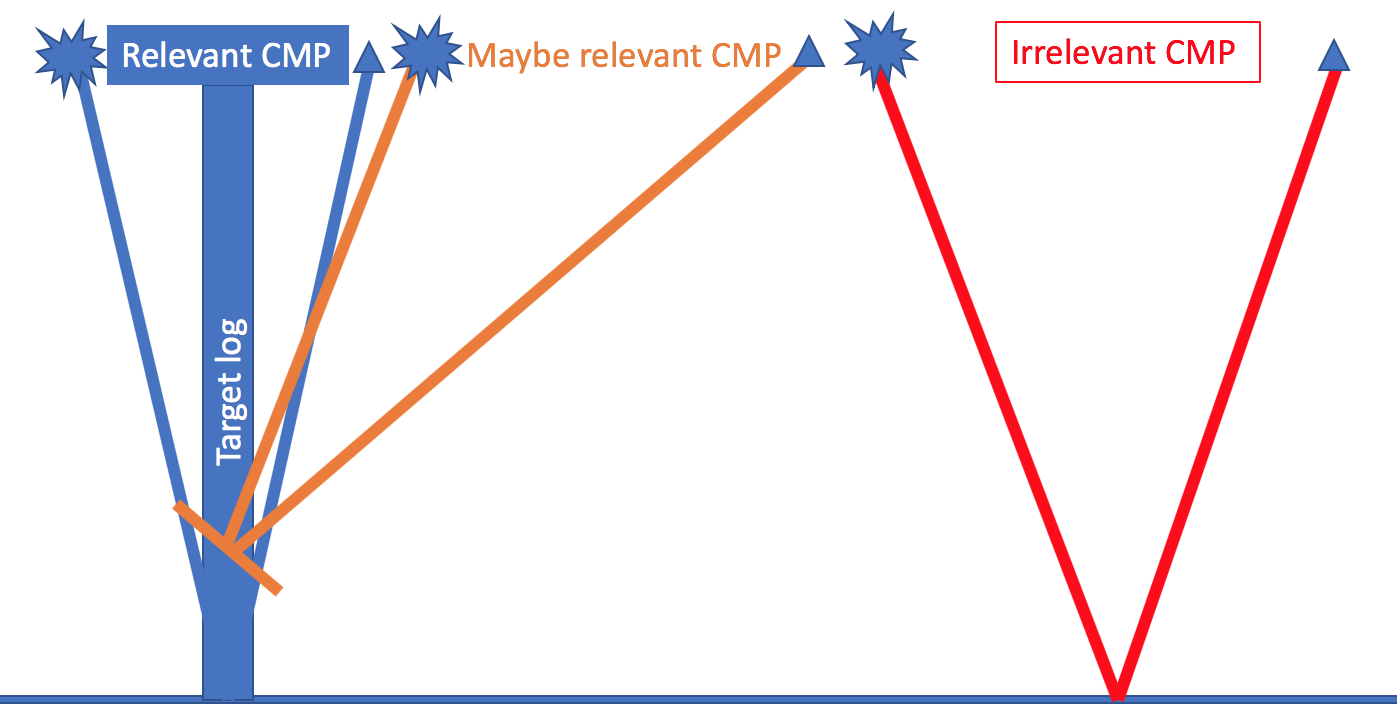
\includegraphics[width=0.7\linewidth]{Fig/relevantCMP}
	\caption{Relevant common mid point (CMP) gathers - right above the image point location are utilized by standard stacking procedures and FWI. The gathers that are slightly shifted may also be useful in laterally heterogeneous media, but they are often discarded. CMP gathers that are far away from the imaging point are not spatially related to the imaging point, we discard those from the input}
	\label{fig:relevantcmp}
\end{figure}

Standard velocity analysis does CMP stacking along hyperbolas and then the stacked data are mapped to depth. This obviously is good enough for horizontally layered media. more advanced velocity analysis techniques such as \todo{crs} or multifocusing take care of mold horizontal velocity variations and curved reflectors relying on curtain assumptions about the subsurface. We purpose to take this concept to it's extreme by relying on geologically plausible models as realistic scenarios and replacing the analysis with deep learning inference.

\subsection{Exploiting the regularity of sampling}
we rely on regularity of conventional seismic exploration data and exploit standard extended velocity analysis approach.  the
the subsurface models for training are generated by another neural network.


\section{Data}
Data-driven applications heavily depend on compound and quantity of samples in the dataset which makes data collection and selection crucial. 
%
We intend to produce virtual well-logs from seismic data arranged into common-midpoint gathers. The dataset for such application should consist of input seismic data and respective target logs. However, there is very limited amount of field samples on well-logs because drilling and collection of a core is a costly task. 
%
To overcome this limitation we generate a synthetic dataset representing real-world geological features. First, we generate a set of random initiations of subsurface models and then numerically propagate seismic waves in them. Later, recorded wavefields are assembled into CMPs and the random velocity models are decomposed into set of well logs.

\subsection{Realistic random models}
Despite the clarity of intention, there is still no a recognized way for generation of realistically textured all-purpose subsurface models with proper geological compound. 
%
We empirically generate slowly laterally varying random subsurface models in three steps. First, we create a prior model which remains the same for the entire dataset. To build the prior, we first laterally stretch Marmousi II benchmark model and then replicate it \figref{stretchMarm}. At the second step, we crop a patch from the prior with target dimensions of the new random model \figref{stretchMarm_strip}. 

\dplot{stretchMarm}{stretchMarm_strip}{To generate a slowly varying laterally model we first stretch the Marmousi II benchmark model laterally and then replicate it. (a) Full prior model. (b) Crop of the prior with dimensions similar to the original Marmousi II model.}


Third, for every new subsurface model we produce a distortion map \figref{deformedModelMild} and stretch the coordinates accordingly \figref{deformedModelNormal}.

\dplot{deformedModelMild}{deformedModelNormal}{Random Gaussian field defines (a) vertical shifts that we apply to the model. (b) deformed model}

The generator described above allows us to generate a set of models which to some extent mimic the layered geological structure from the Marmousi II model. Despite using a specific velocity reference, the generator produces diverse range of subsurface models which then might be fit into desired range of velocities. The main part of the transformation is local texture vertical repositioning. However, depending on smoothness of coordinate transformation new horizontal layers can be generated and old layers collapsed.

\subsection{Seismic wave propagation}
To generate seismic data in each random model we integrate Madagascar package into the workflow. We use a CUDA-accelerated acoustic finite-difference solver in time domain to numerically simulate seismic wave propagation and to record seismograms at each receiver for every source in the acquisition, \figref{X_scaled}.

There are no principal limitations to the type of solver to be used. The proposed data-driven solution is capable of working with data of any complexity. Computational costs of modeling is the only obstacle.

\dplot{T_scaled}{X_scaled}{Scaled version of velocity logs. (b) scaled version of CMP gather. We utilize only positive offset as the data are synthetic and due to the reciprocity there is no difference with swaping source and receiver positions.}


% function "sfgenshots" - a cuda-based finite-difference solver. There are no principal limitations to the type of solver to be used. After that the shots are sorted into CMP gathers.

\section{Deep learning framework}
The general idea of deep learning is to build a mathematical model which would derive a desired non-linear relation directly from the data. Selection of a particular DL model is heavily motivated by the compound and attributes of the available data. 
%	supervised learning
In this study,  pairs of input CSGs and target well-logs \figref{in_out_shape} uniquely define the supervised learning paradigm as the most appropriate. At the training stage, a supervised model attempts to derive a relation which would link input and target variable for each pair in the training partition of the dataset . Whereas at the inference stage, the model infers target variables when given a sample from previously unseen test partition of the data.

\aplot{in_out_shape}{width=0.7\columnwidth}{Shape of input and target data}

\subsection{Convolutional neural network}
%   spatial dependency = convolutional
Regular feed-forward neural networks such as multilayer perceptron are suitable for problems with relatively small size of input data as the number of parameters in them grows exponentially. When the input volume is image then networks with convolutional layers come into play. Convolutional layers perform convolution of the input volume with a set of filters which results in a set of feature maps, one corresponding for each filter respectively. The key feature of convolutional layer is that it features local connectivity. Meaning that when the filter slides over the input volume, only very few neighboring points contribute into particular point of the feature map. This feature allows such a network to learn spatial patterns and enforce them at the inference stage.

\subsection{Preprocessing}
Regardless of the type a DL model used in the application, proper normalization is required for each sample of the input and target data. Proper normalization makes data fit the range matching the bounds of activation functions as well as enforces even contribution of features into training. All these leads weight optimization to a better convergence at shorter time.

In this study, we fit both input and target volumes into range $[-1, 1]$ as well as we set the zero mean.

%


%	Preprocessing
%		explain preprocessing
%	explaing perks of conv 
%	keras tensorflow




Here, following \citep{york2019}, we generate the data and try to learn the respective logs.



\section{Single CMP to single log}
Should the model be horizontally invariant, one can try to reconstruct its elastic layers from a single shot gather \citep{roth1994}, or a single CMP gather \citep{york2019}.
While there is limited domain of applicability to laterally inhomogeneous models \citep{york2019}, to the best of our knowledge, training was always performed on vertically variant models to speed up the data generation. Here we utilize conventional 2D wave propagation and investigate different options for laterally variant media. First we presume that the models are rather smooth laterally.
\subsection{Training data set fitting}


\subsection{Generalization tests}

\paragraph{Guiding model}
The first question that we would like to answer is if the CNN that we trained can fit parts of the stretched Marmousi model that were ulilized to make the training data set, yet were not used in training directly.


\paragraph{More model deformations}
The second question is would it work better if we added more models generated just the way we generated our training data set. In order to do so we generate more models with the same generator and test whether the model can fit those already.

\paragraph{Different for the most part horizontally layered model}
In order to test the generalization power of the trained neural network we test it on data that are modeled in a slice from Overthrust model.


\subsection{Failure}
Here we apply neural network to the Marmousi model stretched three times and not stretched at all.

From the last test we clearly see a rather obvious fact -- single CMP gather can not be mapped into velocity log successfully without assumption of laterally slowly variant medium. We believe that this is a good motivation to study mapping of multiple CMP gathers.

\section{Multiple CMP gathers to a single log}

\section{Conclusions}
For regularly sampled data acquisition the problem of full waveform inversion can be represented as a mapping from 3D data (relevant traces) to single velocity logs. This formulation is not a viable option for conventional FWI implementation. Yet for neural network implementation it is benefiсial to split whole data set into relevant and irrelevant data to speed up training.  
We analyzed the capabilities of CNNs to infer the relation between the data and vertical velocity slices. For very slowly varying laterally models the fitting by single CMP - single velocity log works rather well and there is no need for multi-CMP processing. However for realistically varying with offset models there is need for multi-CMP input. 


\section{ACKNOWLEDGMENTS}

We thank members of the Seismic Modeling and Inversion group (SMI) and the Seismic Wave Analysis Group (SWAG) at KAUST for constructive discussions.
The research reported in this publication was supported by funding from King Abdullah University of Science and Technology (KAUST), Thuwal, 23955-6900, Saudi Arabia.

\append{Appendix example}



\newpage

\bibliographystyle{apalike}  % style file is seg.bst
\bibliography{zotero}

\end{document}